		\begin{objectives}
			In this tutorial you will explore some modelling and results we can obtain using a ``simple'' dimensional analysis coupled with a clever selection of variables.
			
				These problems relate to the following course learning objectives:
				\begin{itemize}\it 
					\item Model with ODEs. \\[-20pt]
					\item Using dimensional analysis to obtain properties of a model.
				\end{itemize}
		\end{objectives}


\vspace{-.5em}
\subsection*{Buckingham Pi Theorem}
\vspace{-.5em}


\begin{definition}[Buckingham Pi Theorem]
	Any physical relation involving $N$ dimensional variables can be written in terms of a complete set of $N - r$ independent dimensionless variables, where $r$ is the rank of the dimensional matrix $\mathcal{D}$.
		
	The notational convention for the Buckingham Pi Theorem is that the ``pi's'', $\Pi_1,\ldots, \Pi_{N-r}$ represent dimensionless variables and a relation between them is given by $F(\Pi_1,\ldots,\Pi_{N-r}) = 0$.
\end{definition}


\vspace{-.5em}
\subsection*{Problems}
\vspace{-.5em}


\begin{enumerate}
	\item\label{q1}\footnote{Based on the 2019 test 1.} Last Thanksgiving I called my mom to ask how long I should roast my 2 kg turkey in the oven. She said 2 hours. Several extra guests were added and I ended up cooking a turkey with mass 8 times larger, 16 kg. Rather than making another call to my mom, we will use \textbf{dimensional analysis} to determine how long I should have cooked the turkey. \\
	
		The heat equation is
		\[
		\frac{\partial T}{\partial \tau} = -\frac{k}{c\rho} \left[ \frac{\partial^2 T}{\partial x^2} + \frac{\partial^2 T}{\partial y^2} + \frac{\partial^2 T}{\partial z^2} \right],
		\]
	where 
	\begin{itemize}
		\item $k = $ thermal conductivity % with units $M L T^{-3} \Theta^{-1}$
		\item $c = $ specific heat % with units $L^2 T^{-2} \Theta^{-1}$
	\end{itemize}

	Because when we change the turkey to a larger one, the mass density doesn't change, we need an explicit expression of the mass into the equation:
	\begin{itemize}
		\item $\rho = m/V$ mass density
		\item $m$ is the mass of the turkey
		\item $V$ is the volume of the turkey
	\end{itemize}

	\begin{enumerate}
		\item Observe that $k$ and $c$ don't relate to our objective: cooking time vs turkey size. So we can define $\beta = \frac{k}{c}$ as a variable. Use the PDE to find its units.
		\item What are the relevant variables we need to consider and what are their units?
		\item What is the dimensional matrix $\mathcal{D}$, its rank and nullity?
		\item Find a bases for its null space.
		\item Use the Buckingham Pi Theorem to conclude a relation between the variables.
		\item Use this relation to find the cooking time of the larger turkey.
		
		\textit{Hint: When you consider the larger turkey, remember that the mass density remains constant. What does this imply?}
	\end{enumerate}

	
	
	
\vfil 


%\newpage

\item \label{q2} \footnote{From the 2022 test 1.} A compressive wave propagates with speed $v$ (a length per time) through a long solid metal bar. The bar has a density $\rho$ (a mass per volume) and a compressive stiffness, known as the Young's modulus, $E$ (a pressure or a force per area).

\begin{enumerate}

	\item Use the Buckingham Pi Theorem to determine a relationship among these three variables.

	\item Use the measurements of the wave speed in various metal bars plotted below to determine any unknown functions.
	
	\hfill
	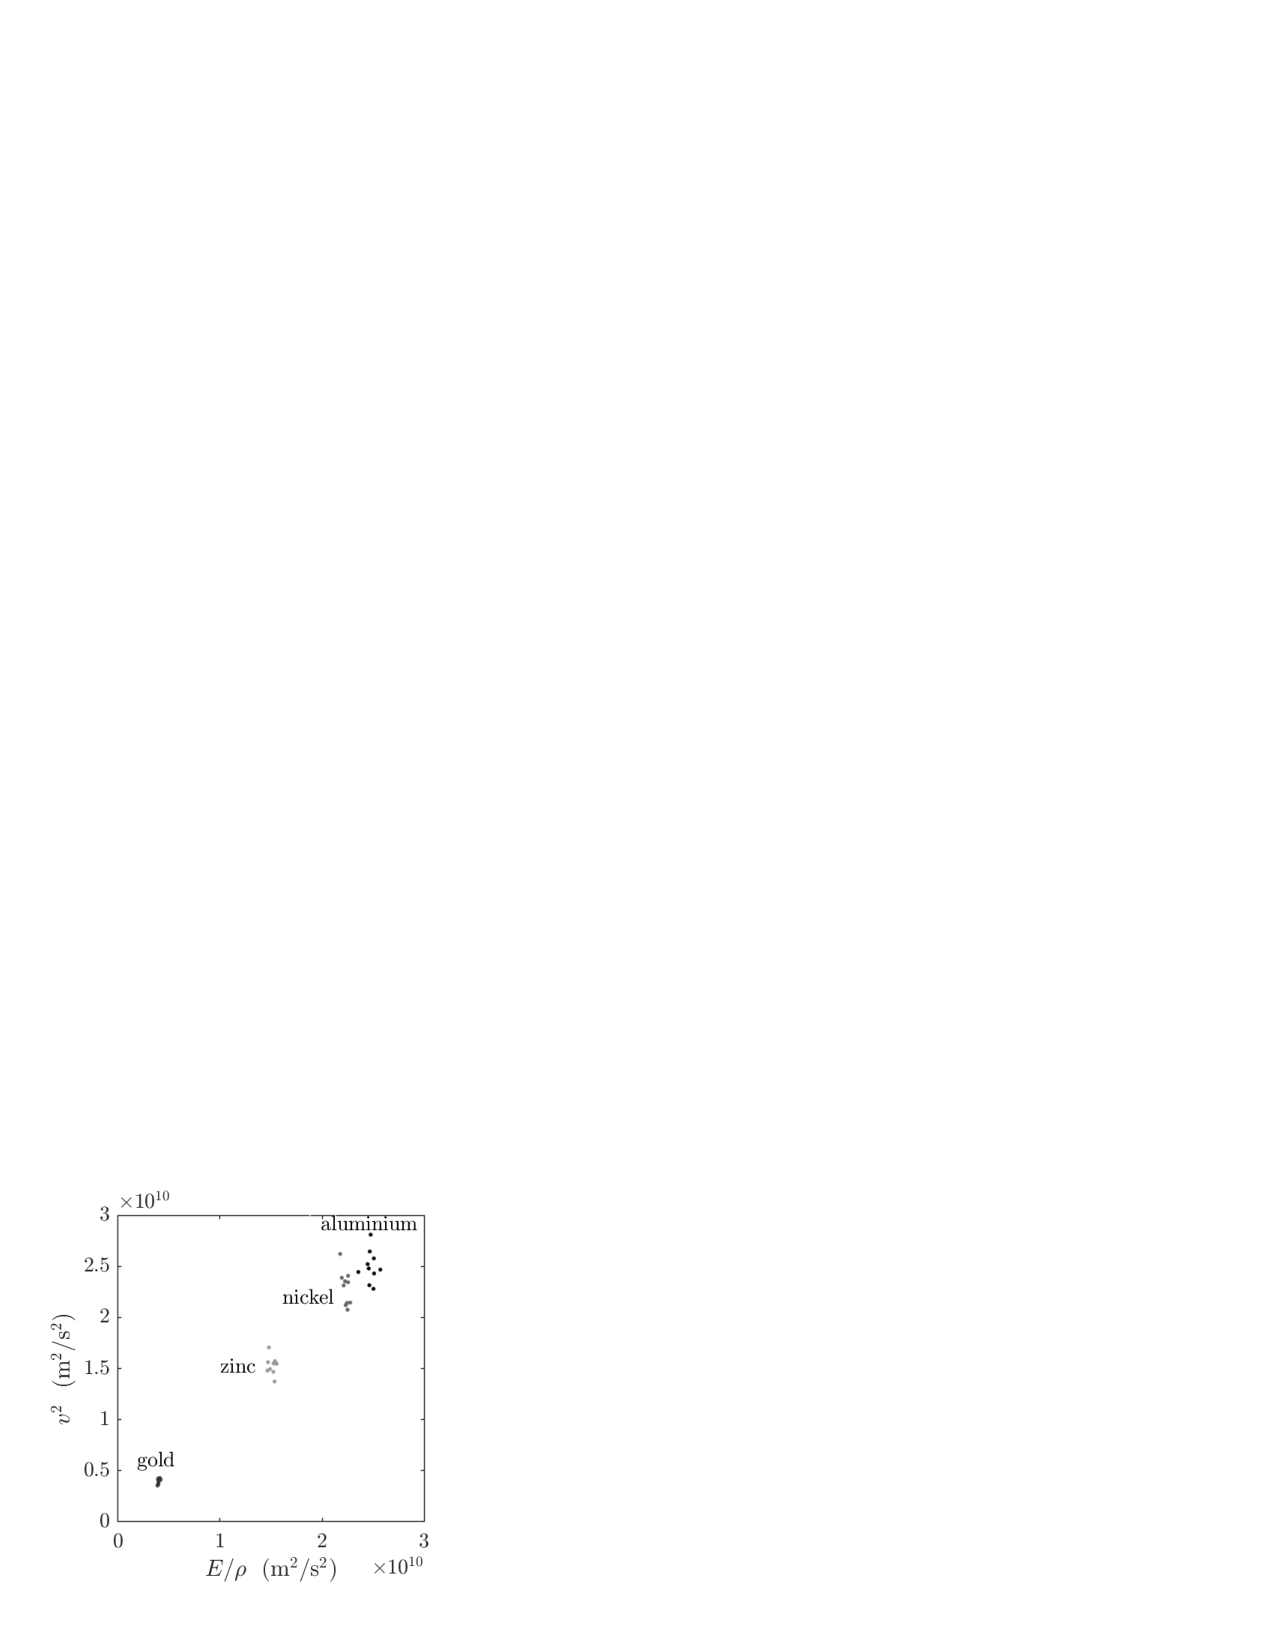
\includegraphics[width=200pt]{WaveSpeed_YoungModulus.pdf}
	
	
\end{enumerate}


\vfil 

\item \label{q3} \textit{(challenge problem)} Find how the speed of a surface wave in deep ocean water is related to its wavelength using dimension analysis. How does doubling the wavelength change the speed of the wave?

\textit{Hint: You have to consider good variables for it to work.}

\end{enumerate}
















